% 
% Lecture Template for ME3050 -  Dynamics Modeling and Controls - Tennessee Technological University
%
% Spring 2020 - Summer 2020
% Tristan Hill, May 07, 2020 - June 12, 2020
% Module 5 - Rotating Systems
% Topic 2 - 
%

%\documentclass{beamer}                         % for presentation (has nav buttons at bottom)
\documentclass[handout]{beamer}  % for handout 
\usepackage{beamerthemesplit}
\usepackage{amsmath}
\usepackage{listings}
\usepackage{multicol}
\usepackage{framed}

\beamertemplateballitem

% custom colors
\definecolor{TTUpurple}{rgb}{0.3098, 0.1607, 0.5176} % TTU Purple (primary)
\definecolor{TTUgold}{rgb}{1.0000, 0.8666, 0.0000} % TTU Gold (primary) 
\definecolor{mygray}{rgb}{.6, .6, .6}
\definecolor{mypurple}{rgb}{0.6,0.1961,0.8}
\definecolor{mybrown}{rgb}{0.5451,0.2706,0.0745}
\definecolor{mygreen}{rgb}{0, .39, 0}
\definecolor{mypink}{rgb}{0.9960, 0, 0.9960}

% color commands
\newcommand{\R}{\color{red}}
\newcommand{\B}{\color{blue}}
\newcommand{\BR}{\color{mybrown}}
\newcommand{\K}{\color{black}}
\newcommand{\G}{\color{mygreen}}
\newcommand{\PR}{\color{mypurple}}
\newcommand{\PN}{\color{mypink}}
\newcommand{\OR}{\color{TTU}}
\newcommand{\GD}{\color{TTUgold}}


\setbeamercolor{palette primary}{bg=TTUpurple,fg=TTUgold}
\setbeamercolor{palette secondary}{bg=black,fg=TTUgold}
\setbeamercolor{palette tertiary}{bg=black,fg=TTUpurple}
\setbeamercolor{palette quaternary}{bg=TTUgold,fg=black}
\setbeamercolor{structure}{fg=TTUpurple} % itemize, enumerate, etc
\setbeamercolor{section in toc}{fg=TTUpurple} % TOC sections

%\usefonttheme{professionalfonts}

\newcommand{\Lagr}{\mathcal{L}} % lagrangian

\newcommand{\hspcu}{\underline{\hspace{20mm}}} % large horizontal space w underline
\newcommand{\vspccc}{\vspace{6mm}\\} % large vertical space
\newcommand{\vspcc}{\vspace{4mm}\\}   % medium vertical space
\newcommand{\vspc}{\vspace{2mm}\\}     % small vertical space

\newcommand{\hspcccc}{\hspace{10mm}} % large horizontal space
\newcommand{\hspccc}{\hspace{6mm}} % large horizontal space
\newcommand{\hspcc}{\hspace{4mm}}   % medium horizontal space
\newcommand{\hspc}{\hspace{2mm}}     % small horizontal space

\newcommand{\eqscl}{0.9}     % small horizontal space


\author{ME3050 - Dynamics Modeling and Controls} % original formatting from Mike Renfro, September 21, 2004

\newcommand{\MNUM}{5\hspace{2mm}} % Module number
\newcommand{\TNUM}{2\hspace{2mm}} % Topic number 
\newcommand{\moduletitle}{Rotation Systems }
\newcommand{\topictitle}{Mass Moment of Inertia} 

\newcommand{\sectiontitleI}{Mathematical Defintion}
\newcommand{\sectiontitleII}{Table of Common Geometries}
\newcommand{\sectiontitleIII}{The Parallel Axis Theorem}
\newcommand{\sectiontitleIV}{Equivalent Inertia}

% custom box
\newsavebox{\mybox}

\title{Module \MNUM - \moduletitle}

\date{Mechanical Engineering\vspc Tennessee Technological University}

\begin{document}

\lstset{language=MATLAB,basicstyle=\ttfamily\small,showstringspaces=false}

\frame{\titlepage \center\begin{framed}\Large \textbf{Topic \TNUM - \topictitle}\end{framed} \vspace{5mm}}

% Section 0: Outline
\frame{

\large \textbf{Topic \TNUM - \topictitle} \vspace{3mm}\\

\begin{itemize}

	\item \sectiontitleI		\vspc % Section I
	\item \sectiontitleII 	\vspc % Section II
	\item \sectiontitleIII 	\vspc %Section III
	\item \sectiontitleIV 	\vspc %Section IV
	
\end{itemize}

}

% Section I:
\section{\sectiontitleI}

% Section I - Frame I
\frame{
\frametitle{\sectiontitleI}

\small
The mass moment of inertia is the combined resistance to angular acceleration from about an axis due to the mass of a body. \vspc

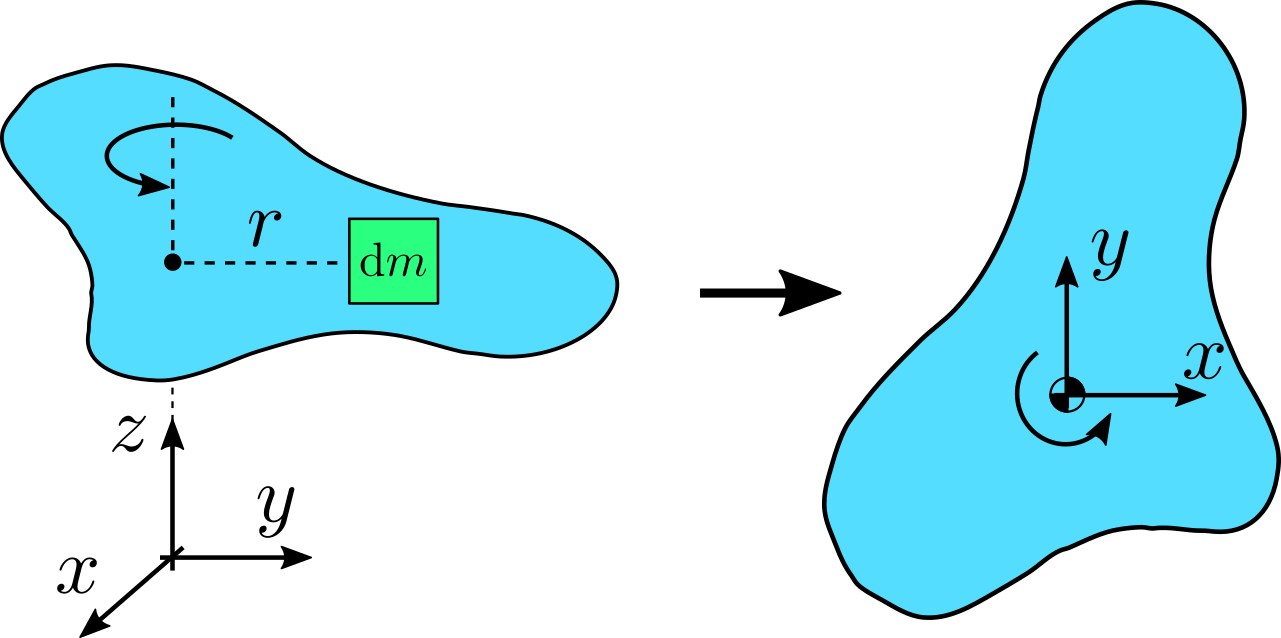
\includegraphics[scale=.225]{moment_inertia_fig3.png} \vspc

\scalebox{.9}{$I=\int\displaylimits_0^M r^2dm$}\vspc

This is done about an axis through the mass center which is also the geometric center for a uniform mass. For planar motion only rotation about the z-axis is considered. 

\vspace{1mm}
{\tiny Image: T. Hill }

}

% Section I - Frame II
\frame{
\frametitle{\sectiontitleI}

\small
If the body is considered as discrete point masses the mass moment of  inertia can be easily found as summation. However we need it for a continuous rigid bodies. \vspc
\begin{multicols}{2}
\vspace*{5mm}

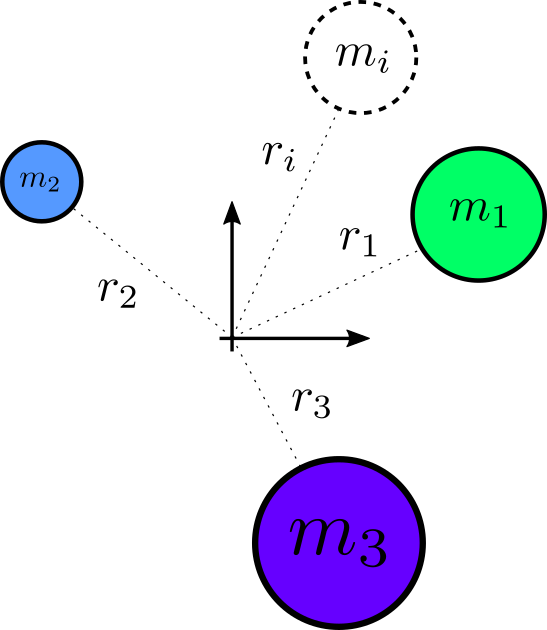
\includegraphics[scale=.225]{moment_inertia_fig2.png} \vspc
\end{multicols}


\vspace{1mm}
{\tiny Image: T. Hill }

}



% Section II:
\section{\sectiontitleII}

% Section II Frame I
\frame{
\frametitle{\sectiontitleII}
\small
In situation where the point mass assumption is not appropriate the mass moment of inertia of common geometries is tabulated.

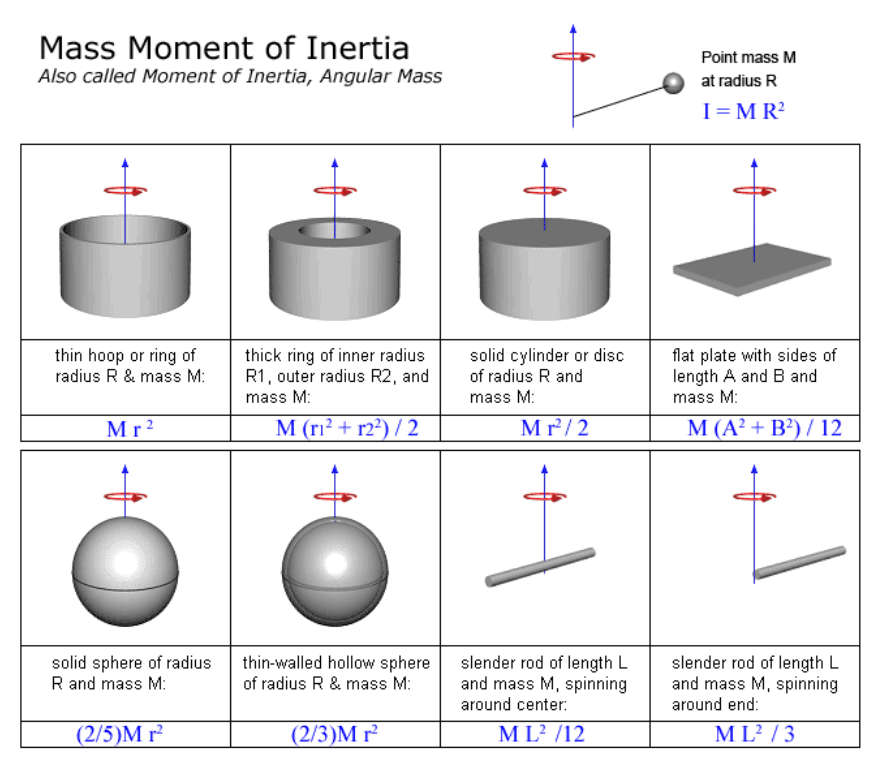
\includegraphics[scale=.225]{moment_inertia_fig1.png}
\vspace{1mm}
{\tiny Images: }

}


% Section III:
\section{\sectiontitleIII}

% Section III Frame I
\frame{
\frametitle{\sectiontitleIII}
\small
Further the object may be rotation about an axis that is removed from the geometrical center. In this situation the moment of inertia about the new axis is found using the \hspcu\hspc\hspcu\hspc\hspcu  \vspc

\begin{multicols}{2}




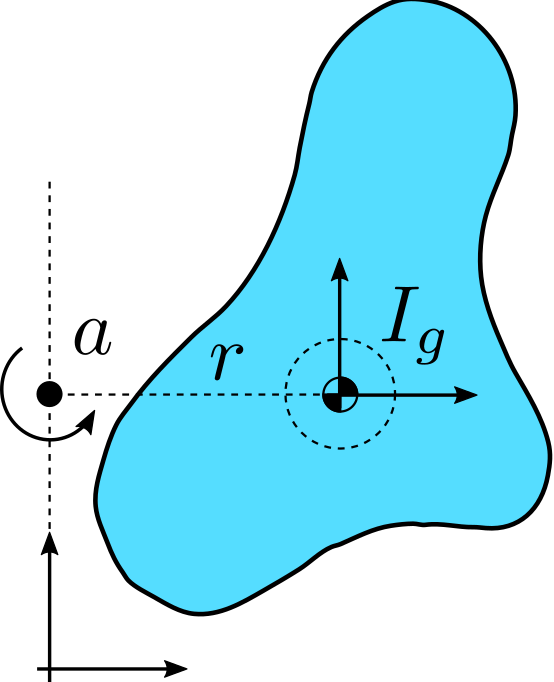
\includegraphics[scale=.225]{moment_inertia_fig4.png}

\end{multicols}

}

% Section IV:
\section{\sectiontitleIV}

% Section IV Frame I
\frame{
\frametitle{\sectiontitleIV}

Some systems composed of translating and rotating parts whose motions are directly coupled can be modeled as as a purely translational or as a purely rotational system, by using the concepts of equivalent mass and inertia. These models can be derived using kinetic energy equivalence.  \vspcc

The textbook discusses several examples we will not discuss this further in ME3050.
 
\vspace{5mm}
{\tiny Text: \underline{System Dynamics, 3rd Edition} , Palm}


}
	
\end{document}





